%!TEX root = ../tesis_mbc.tex

\chapter{Resultados}

Los algoritmos presentados en este trabajo fueron implementados en el lenguaje para cómputo estadístico \texttt{R} \cite{R_manual} y fueron probados con dos conjuntos de datos: \textit{MovieLens}, una página que ofrece recomendaciones de películas \cite{harper2016movielens}; y \textit{BookCrossing}, una plataforma similar, pero enfocada a libros \cite{ziegler2005improving}. Ambos conjuntos de datos están abiertos al público. Algunas de las funciones utilizadas fueron implementadas en el lenguaje \texttt{C++} y compiladas en \texttt{R} con el paquete \texttt{Rcpp} \cite{Rcpp_Book_Eddelbuettel} \cite{Rcpp_Article_Eddelbuettel_Francois}. Las gráficas fueron hechas con \texttt{ggplot2} \cite{wickham_ggplot2} y la manipulación de los datos fue mayoritariamente con los paquetes incluidos en \texttt{tidyverse} \cite{wickham_tidyverse}.

\subsection{Análisis exploratorio de datos}

%%%%%%%%%%%%%%%%%%%%%%%%%%%%%%%%%%%%%%%%%%%%%%%%%%%%%%
%%% MovieLens
%%%%%%%%%%%%%%%%%%%%%%%%%%%%%%%%%%%%%%%%%%%%%%%%%%%%%%

\subsubsection{\textit{MovieLens}}

El conjunto de datos de \textit{MovieLens} consiste en \numprint{20000263} calificaciones de \numprint{26744} películas hechas por \numprint{138493} usuarios. Todos los usuarios habían calificado al menos 20 películas. Las calificaciones están en una escala de $0.5$ a $5$, con intervalos de medio punto, es decir, se puede poner $0.5, 1, \hdots, 4.5, 5$ como calificación. La distribución de las calificaciones se puede ver en la figura \ref{fig:ML_frec_calificaciones}; mientras que en la figura \ref{fig:ML_hist_prom_cals} se puede ver el histograma de los promedios por película.

\begin{figure}[H]
	\centering
 	\includegraphics[width=0.7\textwidth]{frecuencia_calificaciones_MovieLens.pdf}
 	\caption{Frecuencia de calificaciones del conjunto de datos \textit{MovieLens}.}
 	\label{fig:ML_frec_calificaciones}
\end{figure}

\begin{figure}[H]
	\centering
 	\includegraphics[width=0.7\textwidth]{calificacion_promedio_articulo_MovieLens.pdf}
 	\caption{Histograma del promedio de calificaciones por película del conjunto de datos \textit{MovieLens}.}
 	\label{fig:ML_hist_prom_cals}
\end{figure}

En la sección \ref{motivacion} se introduce el concepto de cola larga. En la figura \ref{fig:ML_long_tail} se puede ver cómo este fenómeno ocurre en los datos de \textit{MovieLens}, donde es claro que muy pocas películas tienen una gran cantidad de calificaciones, mientras que muchos artículos tienen pocas calificaciones.

\begin{figure}[H]
	\centering
 	\includegraphics[width=0.8\textwidth]{long_tail_MovieLens.pdf}
 	\caption{Cola larga del conjunto de datos \textit{MovieLens}.}
 	\label{fig:ML_long_tail}
\end{figure}

En el conjunto de datos de \textit{MovieLens}, se tiene disponible la fecha en que se hizo la calificación. Como se mencionó antes, esta temporalidad podría ser utilizada en el modelo, pero en este trabajo se decidió no usarlo. En la figura \ref{fig:ML_calis_semana} se muestra la calificación promedio de todas las películas en cada semana. Se puede ver que la calificación promedio no ha cambiado drásticamente, sin embargo se aprecia que tienen forma de U, siendo el mínimo cerca de 2005.

\begin{figure}[H]
	\centering
 	\includegraphics[width=\textwidth]{calificaciones_promedio_semana_MovieLens.pdf}
 	\caption{Calificación promedio semanal de todas las películas del conjunto de datos \textit{MovieLens}.}
 	\label{fig:ML_calis_semana}
\end{figure}

%%%%%%%%%%%%%%%%%%%%%%%%%%%%%%%%%%%%%%%%%%%%%%%%%%%%%%
%%% BookCrossing
%%%%%%%%%%%%%%%%%%%%%%%%%%%%%%%%%%%%%%%%%%%%%%%%%%%%%%

\subsubsection{\textit{BookCrossing}}

El conjunto de datos de \textit{BookCrossing} consiste en \numprint{1149780} calificaciones de \numprint{271379} libros hechas por \numprint{278858} usuarios. Los datos se obtuvieron durante cuatro semanas de agosto a septiembre de 2004. Las calificaciones están en una escala de $1$ a $10$, con intervalos de un punto, es decir, se puede poner $1, 2, \hdots, 9, 10$ como calificación. Se tiene como calificación especial el $0$, el cual es solamente una calificación implícita, es decir, si leyó o no el libro. Debido a que para usar el método presentado en este trabajo se necesitan calificaciones explícitas, se filtraron estas del conjunto de datos original. Con esta operación, quedaron \numprint{383852} calificaciones de \numprint{153683} libros hechas por \numprint{68092} usuarios. La distribución de las calificaciones filtradas se puede ver en la figura \ref{fig:BC_frec_calificaciones}; mientras que en la figura \ref{fig:BC_hist_prom_cals} se puede ver el histograma de los promedios por libro.

\begin{figure}[H]
	\centering
 	\includegraphics[width=0.7\textwidth]{frecuencia_calificaciones_BookCrossing.pdf}
 	\caption{Frecuencia de calificaciones del conjunto de datos \textit{BookCrossing}.}
 	\label{fig:BC_frec_calificaciones}
\end{figure}

\begin{figure}[H]
	\centering
 	\includegraphics[width=0.7\textwidth]{calificacion_promedio_articulo_BookCrossing.pdf}
 	\caption{Histograma del promedio de calificaciones por película del conjunto de datos \textit{BookCrossing}.}
 	\label{fig:BC_hist_prom_cals}
\end{figure}

En la figura \ref{fig:BC_long_tail} se puede ver la cola larga en los datos de \textit{BookCrossing}, donde nuevamente es claro que muy pocas películas tienen una gran cantidad de calificaciones, mientras que muchos artículos tienen pocas calificaciones.

\begin{figure}[H]
	\centering
 	\includegraphics[width=0.8\textwidth]{long_tail_BookCrossing.pdf}
 	\caption{Cola larga del conjunto de datos \textit{BookCrossing}.}
 	\label{fig:BC_long_tail}
\end{figure}

%%%%%%%%%%%%%%%%%%%%%%%%%%%%%%%%%%%%%%%%%%%%%%%%%%%%%%
%%% Comparación
%%%%%%%%%%%%%%%%%%%%%%%%%%%%%%%%%%%%%%%%%%%%%%%%%%%%%%

\subsection{Comparación de modelos}

Para cada conjunto de datos se calculó un modelo base como el descrito en la sección \ref{sec:modelo_base} en la ecuación \ref{ec:modelo_base} y un modelo de factorización como descrito en la sección \ref{sec:modelo_factorizacion}. Cada uno de los conjuntos de datos se dividió en tres subconjuntos: un conjunto de entrenamiento, un conjunto de prueba y un conjunto de validación. Los parámetros de los modelos fueron estimados usando el conjunto de entrenamiento. En el caso del modelo de factorización, el conjunto de validación fue utilizado para estimar el error de predicción y poder utilizarlo como criterio de paro en el algoritmo de optimización y así evitar el sobreajuste. Para el modelo base, el conjunto de validación no fue utilizado, los errores que se muestran en relación con este conjunto son con el conjunto de prueba. La medida de error utilizada fue la raíz del error cuadrático medio (RMSE), definido en la ecuación \ref{ec:rmse}. De aquí en adelante, cuando se hable de error, es con referencia a la raíz del error cuadrático medio.

%%%%%%%%%%%%%%%%%%%%%%%%%%%%%%%%%%%%%%%%%%%%%%%%%%%%%%
%%% MovieLens
%%%%%%%%%%%%%%%%%%%%%%%%%%%%%%%%%%%%%%%%%%%%%%%%%%%%%%

\subsubsection{\textit{MovieLens}}

Para \textit{MovieLens}, el número de usuarios, artículos y calificaciones en cada uno de los conjuntos se puede ver en la tabla \ref{tab:ML_num_art_usu_cal}.

\begin{table}[H]
	\centering
	\caption{Número de usuarios, calificaciones y artículos en los conjuntos de \textit{MovieLens}.}
	\label{tab:ML_num_art_usu_cal}
	\begin{tabular}{|l|l|l|l|}
		\hline
		Conjunto      & Número de artículos & Número de usuarios & Número de calificaciones \\ \hline
		Entrenamiento & \numprint{26247}               & \numprint{138493}             & \numprint{18029206} \\ \hline
		Validación    & \numprint{6256}                & \numprint{41483}              & \numprint{1469158} \\ \hline
		Prueba        & \numprint{2895}                & \numprint{20676}              & \numprint{501899} \\  \hline
	\end{tabular}
\end{table}

En la figura \ref{fig:ML_modelo_base_errores} se pueden ver los errores del modelo base en el conjunto de prueba, de acuerdo al valor del parámetro de regularización $\gamma$, definido en la ecuación \ref{ec:modelo_base}. Se puede ver que con $\gamma \approx 19$ se minimiza el valor de la raíz del error cuadrático medio en el conjunto de prueba, siendo este de aproximadamente 0.8707.

\begin{figure}[H]
	\centering
 	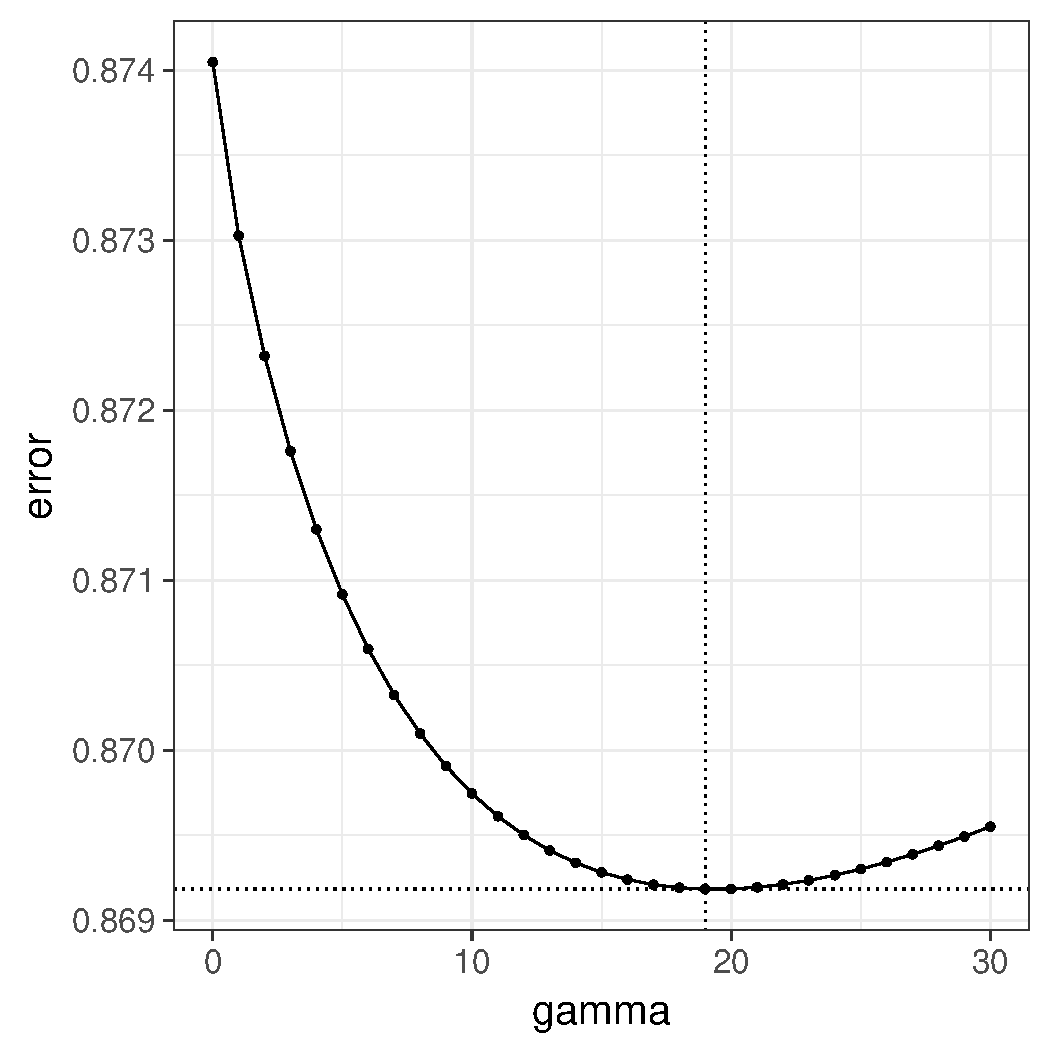
\includegraphics[width=0.7\textwidth]{modelo_base_MovieLens.pdf}
 	\caption{Errores del modelo base en el conjunto de prueba de \textit{MovieLens}, de acuerdo al valor del parámetro de regularización $\gamma$.}
 	\label{fig:ML_modelo_base_errores}
\end{figure}

En la figura \ref{fig:ML_modelo_fact_errores} se pueden ver los errores de entrenamiento y de validación del modelo de factorización con distintos valores en el número de dimensiones latentes, tasa de aprendizaje y parámetro de regularización $\lambda$. Como es de esperarse, el error de entrenamiento es menor en cada uno de los casos. También se podría esperar que mientras más dimensiones latentes haya, el error de entrenamiento sea menor, debido a que hay más dimensiones para aproximar la matriz que se quiere aproximar; y es justo lo que sucede: los modelos con más dimensiones latentes tienen menor error de entrenamiento. Sin embargo, se sabe que menor error de entrenamiento no implica necesariamente menor error de validación; por lo que se busca el modelo con menor error de validación. En este caso, todos los modelos tienen un error de validación relativamente parecido, siendo el de $500$ dimensiones latentes, tasa de aprendizaje de $0.001$ y $\lambda = 0.01$ el modelo con menor error ($0.763325$), siguiendo el de $200$ dimensiones latentes, tasa de aprendizaje de $0.001$ y $\lambda = 0.01$ con un error de $0.765166$. 

Aquí se podría tomar una decisión en cuanto a qué modelo utilizar: el modelo con $500$ dimensiones latentes tiene menor error, pero tiene más del doble de dimensiones latentes que el de $200$, el cual tiene un desempeño muy parecido, por lo que tal vez se preferiría utilizar el modelo con $200$ dimensiones latentes debido a que es más simple y tiene casi el mismo desempeño. El modelo que se utilizó como final fue el de $200$ dimensiones latentes, con un error en el conjunto de prueba de $0.7651675$ (muy parecido al del conjunto de validación). Se hace notar que en todos los casos, el algoritmo de factorización presenta un error menor que el modelo base.

\begin{figure}[H]
	\centering
 	\includegraphics[width=0.85\textwidth]{errores_ent_validacion_factorizacion_MovieLens.pdf}
 	\caption{Errores del modelo de factorización en el conjunto de prueba de \textit{MovieLens}. LR es la tasa de aprendizaje, DL es el número de dimensiones latentes y L es el parámetro de regularización $\lambda$.}
 	\label{fig:ML_modelo_fact_errores}
\end{figure}

En la figura \ref{fig:ML_modelo_fact_error_por_iter} se pueden ver los errores de entrenamiento y de validación del modelo de factorización final (i.e., $200$ dimensiones latentes, tasa de aprendizaje de $0.001$ y $\lambda = 0.01$) en cada iteración del algoritmo de descenso en gradiente estocástico. Se puede ver cómo ambos errores disminuyen con cada iteración, sin embargo, el error de entrenamiento disminuye mucho más rápido. Si no se hubiera tenido como criterio de paro el error de validación, posiblemente el error de entrenamiento hubiera continuado disminuyendo, pero el de validación hubiera empezado a aumentar, debido al sobreajuste.


\begin{figure}[H]
	\centering
 	\includegraphics[width=0.8\textwidth]{error_por_iteracion_modelo_fact_MovieLens.pdf}
 	\caption{Errores de entrenamiento y validación del modelo de factorización en cada iteración del algoritmo de optimización para \textit{MovieLens}.}
 	\label{fig:ML_modelo_fact_error_por_iter}
\end{figure}

Como se menciona en \ref{sec:evaluacion_modelos}, además del RMSE, una forma de evaluar un sistema de recomendación es como un problema de clasificación con la tarea de recomendar los mejores $N$ artículos. En las figuras \ref{fig:ML_recall_top_N} y \ref{fig:ML_precision_top_N} se puede ver el resultado de esta tarea comparando el modelo base y el modelo de factorización como función de $N$, el número de artículos recomendados. Se puede observar que el modelo de factorización es superior que el modelo base para todas las $N$ para las que se calcularon las medidas. Por ejemplo, para $N = 10$, el recall del modelo de factorización es de 0.429, lo cual significa que el modelo tiene una probabilidad de 0.429 de poner en el top-10 de recomendaciones una película que atraiga a un usuario; mientras que el recall del modelo base en $N = 10$ es de 0.059, lo cual significa que la probabilidad mencionada es de 0.059.

\begin{figure}[H]
	\centering
 	\includegraphics[width=0.8\textwidth]{recall_base_fact_MovieLens.pdf}
 	\caption{Recall para cada valor de $N$ en la tarea de las mejores $N$ recomendaciones para \textit{MovieLens}.}
 	\label{fig:ML_recall_top_N}
\end{figure}

\begin{figure}[H]
	\centering
 	\includegraphics[width=0.8\textwidth]{precision_base_fact_MovieLens.pdf}
 	\caption{Precisión para cada valor de $N$ en la tarea de las mejores $N$ recomendaciones para \textit{MovieLens}.}
 	\label{fig:ML_precision_top_N}
\end{figure}

Como se mencionó antes, cada artículo es expresado como una combinación lineal de distintos factores latentes, por lo que artículos y usuarios son mapeados a un mismo espacio latente. Por ende, cada artículo tiene un vector representante en un espacio euclidiano, por lo que se pueden calcular distancias y encontrar vecinos con estas distancias. Con esta idea, además de recomendar directamente a un usuario artículos personalizados, se pueden encontrar los artículos más parecidos a un determinado artículo mediante la norma euclidiana de la diferencia o la similitud coseno. 

Para el conjunto de datos de \textit{MovieLens} se calculan los vecinos más cercanos para algunas películas selectas. Se utilizó la distancia euclidiana y se calculó con el paquete \texttt{RANN} \cite{RANN_package} de \texttt{R}. Estos vecinos se pueden ver en las tablas \ref{tab:ML_vecinos_cercanos_1} y \ref{tab:ML_vecinos_cercanos_2}, y se puede apreciar que en cierta forma, los vecinos más cercanos de cada película sí son parecidos.

\begin{table}[H]
	\centering
	\caption{Algunas películas y sus vecinos más cercanos.}
	\label{tab:ML_vecinos_cercanos_1}
	\begin{tabular}{ |l|l|l| }
		%\hline
		%\multicolumn{3}{ |c| }{Vecinos} \\
		\hline
		\textbf{Película} & \textbf{Película más cercana} & \textbf{Distancia} \\ \hline
		\multirow{10}{*}{ Aladdin (1992) } &  Lion King, The (1994)  &  1.74  \\
		 &  Beauty and the Beast (1991)  &  1.79  \\
		 &  Little Mermaid, The (1989)  &  2.09  \\
		 &  Princess and the Frog, The (2009)  &  2.33  \\
		 &  Tarzan (1999)  &  2.42  \\
		 &  Mulan (1998)  &  2.43  \\
		 &  Oliver \& Company (1988)  &  2.47  \\
		 &  Great Mouse Detective, The (1986)  &  2.47  \\
		 &  How to Train Your Dragon 2 (2014)  &  2.49  \\
		 &  Anastasia (1997)  &  2.49  \\
		\hline
		\multirow{10}{*}{ Hannibal (2001) } &  Red Dragon (2002)  &  2.58  \\
		 &  Hitcher, The (2007)  &  2.88  \\
		 &  Venom (2005)  &  2.89  \\
		 &  Quiet, The (2005)  &  2.89  \\
		 &  Hannibal Rising (2007)  &  2.89  \\
		 &  Mindhunters (2004)  &  2.9  \\
		 &  187 (One Eight Seven) (1997)  &  2.91  \\
		 &  Raven, The (2012)  &  2.91  \\
		 &  Taking Lives (2004)  &  2.93  \\
		 &  Don't Say a Word (2001)  &  2.93  \\
		\hline
		\multirow{10}{*}{ \shortstack{Harry Potter and the \\ Sorcerer's Stone (2001)} } &  HP and the Chamber of Secrets (2002)  &  0.47  \\
		 &  HP and the Prisoner of Azkaban (2004)  &  1.11  \\
		 &  HP and the Goblet of Fire (2005)  &  1.13  \\
		 &  HP and the Order of the Phoenix (2007)  &  1.33  \\
		 &  HP and the Half-Blood Prince (2009)  &  1.59  \\
		 &  HP and the Deathly Hallows: Part 2 (2011)  &  1.83  \\
		 &  HP and the Deathly Hallows: Part 1 (2010)  &  1.87  \\
		 &  Narnia: The Voyage of the Dawn Treader (2010)  &  2.76  \\
		 &  Narnia: Prince Caspian (2008)  &  2.88  \\
		 &  The Lion King 1 1/2 (2004)  &  2.91  \\
		\hline
	\end{tabular}
\end{table}


\begin{table}[H]
	\centering
	\caption{Algunas películas y sus vecinos más cercanos.}
	\label{tab:ML_vecinos_cercanos_2}
	\begin{tabular}{ |l|l|l| }
		%\hline
		%\multicolumn{3}{ |c| }{Vecinos} \\
		\hline
		\textbf{Película} & \textbf{Película más cercana} & \textbf{Distancia} \\ \hline
		\multirow{10}{*}{ Lion King, The (1994) } &  Aladdin (1992)  &  1.74  \\
		 &  Beauty and the Beast (1991)  &  2.1  \\
		 &  Mulan (1998)  &  2.4  \\
		 &  Little Mermaid, The (1989)  &  2.42  \\
		 &  Tarzan (1999)  &  2.44  \\
		 &  Oliver \& Company (1988)  &  2.44  \\
		 &  Princess and the Frog, The (2009)  &  2.48  \\
		 &  Frozen (2013)  &  2.49  \\
		 &  Land Before Time, The (1988)  &  2.49  \\
		 &  How to Train Your Dragon 2 (2014)  &  2.55  \\
		\hline
		\multirow{10}{*}{ Pulp Fiction (1994) } &  Reservoir Dogs (1992)  &  2.26  \\
		 &  Inglorious Bastards (1978)  &  3.03  \\
		 &  Goodfellas (1990)  &  3.15  \\
		 &  An Evening with Kevin Smith 2 (2006)  &  3.19  \\
		 &  Black Mirror (2011)  &  3.2  \\
		 &  Ricky Gervais Live 3: Fame (2007)  &  3.23  \\
		 &  Nightcrawler (2014)  &  3.24  \\
		 &  Inside Llewyn Davis (2013)  &  3.25  \\
		 &  Flirting (1991)  &  3.25  \\
		 &  Generation Kill (2008)  &  3.25  \\
		\hline
		\multirow{10}{*}{ Toy Story (1995) } &  Toy Story 2 (1999)  &  1.43  \\
		 &  Monsters, Inc. (2001)  &  1.91  \\
		 &  Toy Story 3 (2010)  &  2  \\
		 &  Bug's Life, A (1998)  &  2.02  \\
		 &  Finding Nemo (2003)  &  2.03  \\
		 &  Incredibles, The (2004)  &  2.26  \\
		 &  Up (2009)  &  2.47  \\
		 &  For the Birds (2000)  &  2.5  \\
		 &  Wreck-It Ralph (2012)  &  2.5  \\
		 &  Partly Cloudy (2009)  &  2.5  \\
		\hline
	\end{tabular}
\end{table}




%%%%%%%%%%%%%%%%%%%%%%%%%%%%%%%%%%%%%%%%%%%%%%%%%%%%%%
%%% BookCrossing
%%%%%%%%%%%%%%%%%%%%%%%%%%%%%%%%%%%%%%%%%%%%%%%%%%%%%%

\subsubsection{\textit{BookCrossing}}

En esta subsección se presentan los mismos resultados en el mismo orden que en la sección anterior para \textit{BookCrossing}. El número de usuarios, artículos y calificaciones en cada uno de los conjuntos se puede ver en la tabla \ref{tab:BC_num_art_usu_cal}.

\begin{table}[H]
	\centering
	\caption{Número de usuarios, calificaciones y artículos en los conjuntos de \textit{BookCrossing}.}
	\label{tab:BC_num_art_usu_cal}
	\begin{tabular}{|l|l|l|l|}
		\hline
		Conjunto      & Número de artículos & Número de usuarios & Número de calificaciones \\ \hline
		Entrenamiento & \numprint{140807}               & \numprint{64459}             & \numprint{351217} \\ \hline
		Validación    & \numprint{13072}                & \numprint{5332}              & \numprint{21224} \\ \hline
		Prueba        & \numprint{5065}                & \numprint{2286}              & \numprint{7435} \\  \hline
	\end{tabular}
\end{table}


En la figura \ref{fig:BC_modelo_base_errores} se pueden ver los errores del modelo base en el conjunto de prueba, de acuerdo al valor del parámetro de regularización $\gamma$, definido en la ecuación \ref{ec:modelo_base}. Se puede ver que con $\gamma \approx 6$ se minimiza el valor de la raíz del error cuadrático medio en el conjunto de prueba, siendo este de aproximadamente 1.7022.

\begin{figure}[H]
	\centering
 	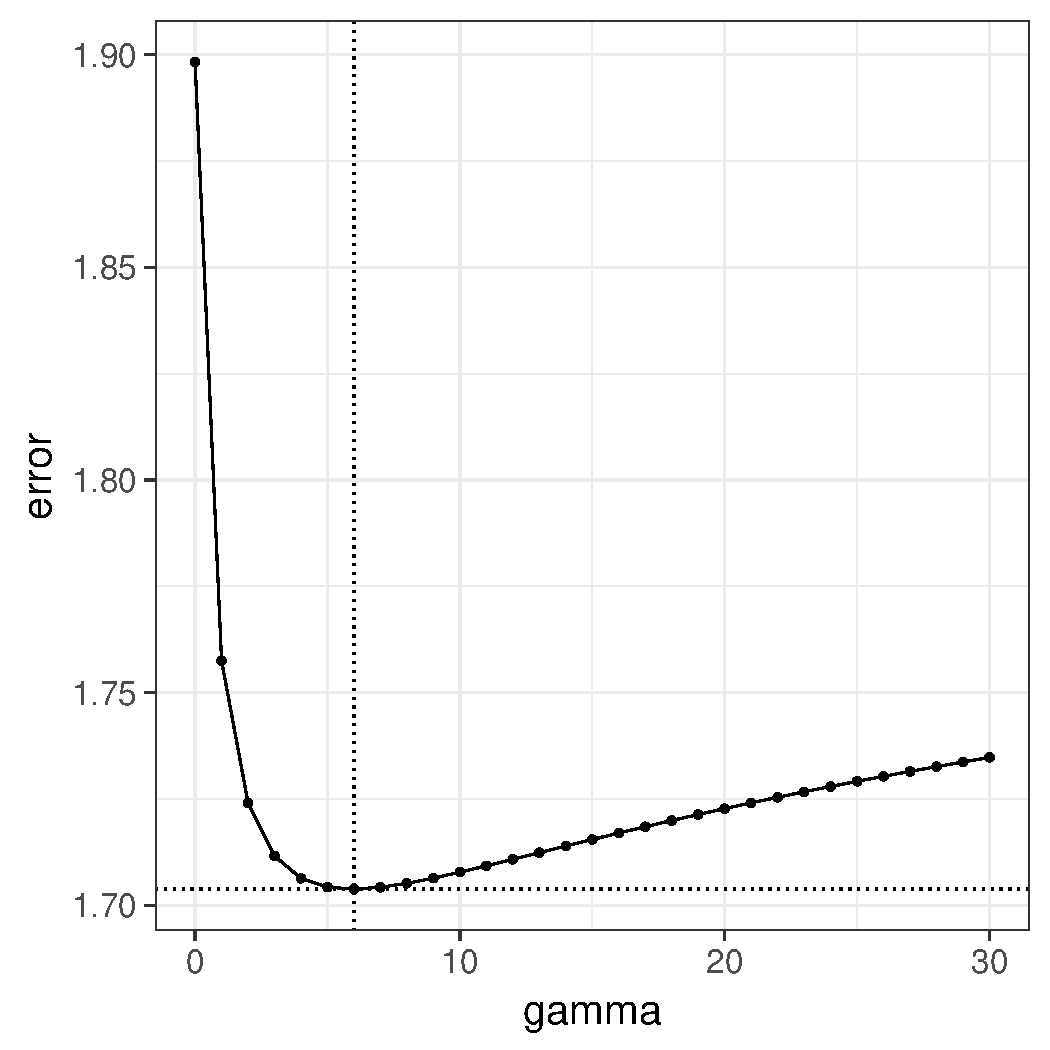
\includegraphics[width=0.7\textwidth]{modelo_base_BookCrossing.pdf}
 	\caption{Errores del modelo base en el conjunto de prueba de \textit{BookCrossing}, de acuerdo al valor del parámetro de regularización $\gamma$.}
 	\label{fig:BC_modelo_base_errores}
\end{figure}

En el caso de \textit{BookCrossing}, el modelo de factorización utilizado y para el cual se presentan resultados es, al igual que con \textit{MovieLens}, uno con $200$ dimensiones latentes, tasa de aprendizaje de $0.001$ y $\lambda = 0.01$. Este modelo presentó con un error en el conjunto de prueba de $1.586566$. Nuevamente, este error es menor al error del modelo base.

En la figura \ref{fig:BC_modelo_fact_error_por_iter} se puede ver, como en la subsección anterior, los errores de entrenamiento y de validación del modelo de factorización final en cada iteración del algoritmo de optimización.

\begin{figure}[H]
	\centering
 	\includegraphics[width=0.8\textwidth]{error_por_iteracion_modelo_fact_BookCrossing.pdf}
 	\caption{Errores de entrenamiento y validación del modelo de factorización en cada iteración del algoritmo de optimización para \textit{BookCrossing}.}
 	\label{fig:BC_modelo_fact_error_por_iter}
\end{figure}

En las figuras \ref{fig:BC_recall_top_N} y \ref{fig:BC_precision_top_N} se puede ver el desempeño del modelo base y del modelo de factorización como problema de clasificación y como función de $N$ (el número de artículos recomendados). Nuevamente, el modelo de factorización es superior que el modelo base para todas las $N$ para las que se calcularon las medidas. Si se compara con el desempeño del conjunto de datos de \textit{MovieLens}, los resultados son mucho peores en este caso. Por ejemplo, para $N = 10$, el recall del modelo de factorización de \textit{MovieLens} es de 0.429, mientras que el del modelo de factorización de \textit{BookCrossing} es de 0.1144. Aún así, en la tarea de recomendar artículos, el algoritmo de factorización supera al modelo base. En el caso de $N = 10$, el modelo base presenta un recall de aproximadamente 0.008, menos de una décima parte que el de factorización.

\begin{figure}[H]
	\centering
 	\includegraphics[width=0.8\textwidth]{recall_base_fact_BookCrossing.pdf}
 	\caption{Recall para cada valor de $N$ en la tarea de las mejores $N$ recomendaciones para \textit{BookCrossing}.}
 	\label{fig:BC_recall_top_N}
\end{figure}

\begin{figure}[H]
	\centering
 	\includegraphics[width=0.8\textwidth]{precision_base_fact_BookCrossing.pdf}
 	\caption{Precisión para cada valor de $N$ en la tarea de las mejores $N$ recomendaciones para \textit{BookCrossing}.}
 	\label{fig:BC_precision_top_N}
\end{figure}

Para el conjunto de datos de \textit{BookCrossing} también se calculan los vecinos más cercanos para algunos libros mediante distancia euclidiana y con el paquete \texttt{RANN}. Los resultados se pueden ver en la tabla \ref{tab:BC_vecinos_cercanos}. Nótese que en este caso, aunque sí se puede apreciar similitud, no es tanta como en el caso de \textit{MovieLens}. Esto se debe a que el conjunto de datos de \textit{BookCrossing} es mucho más ralo.

\begin{table}[H]
	\centering
	\caption{Algunos libros y sus vecinos más cercanos.}
	\label{tab:BC_vecinos_cercanos}
	\begin{tabular}{ |l|l|l| }
		%\hline
		%\multicolumn{3}{ |c| }{Vecinos} \\
		\hline
		\textbf{Libro} & \textbf{Libro más cercano} & \textbf{Distancia} \\ \hline
		\multirow{10}{*}{ \shortstack{Harry Potter \\and the \\Sorcerer's Stone} } &  Who in Hell Is Wanda Fuca?  &  1.71  \\
		 &  A Ranking of the Most Influential Persons in History  &  1.75  \\
		 &  Harry Potter and the Goblet of Fire (Book 4)  &  1.77  \\
		 &  Surviving Production: The Art of Production ...  &  1.77  \\
		 &  Just Tell Me When We're Dead  &  1.79  \\
		 &  The Conquest  &  1.8  \\
		 &  The Ghosts of Cougar Island  &  1.8  \\
		 &  Dr. Death (Alex Delaware Novels (Paperback))  &  1.81  \\
		 &  Familiar Obsession (Fear Familiar) (Intrigue, 570)  &  1.81  \\
		 &  My Gal Sunday  &  1.81  \\
		\hline
		\multirow{10}{*}{ \shortstack{The Catcher \\in the Rye} } &  Soul Stories  &  4.18  \\
		 &  Enchanting Baby The Birth Place &  4.18  \\
		 &  The Road To Echo Point  &  4.29  \\
		 &  The Rosewood Casket  &  4.3  \\
		 &  The Real Allie Newman &  4.32  \\
		 &  Holman Concise Topical Concordance  &  4.35  \\
		 &  East of Eden  &  4.36  \\
		 &  No Lesser Plea  &  4.36  \\
		 &  Juxtaposition (Apprentice Adept)  &  4.37  \\
		 &  Jane Eyre (Puffin Classics)  &  4.37  \\
		\hline
		\multirow{10}{*}{ \shortstack{The Fellowship\\ of the Ring} } &  I Hate Texas: 303 Reasons Why You Should, Too &  0.69  \\
		 &  King Lear  &  0.73  \\
		 &  When Your Marriage Needs Repair &  0.73  \\
		 &  365 Things Every Couple Should Know  &  0.73  \\
		 &  So You Want to Be a Witch  &  0.74  \\
		 &  Keeping of Customers: A Treasury of Facts, Tips \& ...  &  0.74  \\
		 &  Zin! Zin! Zin! A Violin  &  0.74  \\
		 &  Midsummer Nights Dream  &  0.75  \\
		 &  Pinky And Rex And The Mean Old Witch  &  0.75  \\
		 &  Miss Nelson Is Missing!  &  0.75  \\
		\hline
	\end{tabular}
\end{table}



